\documentclass[11pt]{article}

\usepackage[utf8]{inputenc}
\usepackage[T1]{fontenc}
\usepackage[margin=1in]{geometry}
\usepackage{amsmath,amssymb}
\usepackage{enumitem}
\usepackage{tikz}
\usetikzlibrary{positioning}
\usepackage[colorlinks=true,linkcolor=black,citecolor=blue,urlcolor=blue]{hyperref}

\setlist{itemsep=2pt,topsep=4pt,parsep=0pt}

\title{Non-equilibrium effects in Hypermassive Neutron-Star Remnants:\\[2pt]
A BDNK Implementation Plan}
% \author{Your Name \\ California Institute of Technology}
\author{}
\date{\today}

\begin{document}
\maketitle

\begin{abstract}
The aim is to quantify the effect of bulk viscosity, shear viscosity, and heat
conduction on the dynamical evolution and oscillation spectrum of a hot,
out-of-equilibrium hypermassive neutron-star remnant, using the causal, locally
well-posed first-order (BDNK) formulation rather than the acausal
Eckart/Navier--Stokes limit. The program proceeds in three stages:
(i)~reproduction of known results;
(ii)~a $1{+}1$D BDNK code coupled to dynamical general relativity with
baryon-number conservation and a realistic equation of state, targeting the
first BDNK viscous spherical collapse; and (iii)~a $3{+}1$D BDNK code in the
Cowling approximation to resolve non-radial modes. This document records the
scientific motivation, the dependency structure of the build, the
stage-by-stage technical choices, and a phased schedule with validation gates.
\end{abstract}

\section{Scientific motivation}
A post-merger hypermassive remnant, in the interval before it relaxes to
equilibrium, supports shear layers and large-amplitude pulsations; on these
timescales non-equilibrium transport is dynamically relevant rather than a small
correction. The central question is whether dissipation changes (a)~the radial
and collapse stability and (b)~the non-radial mode content of the remnant,
computed in a framework that remains causal and strongly hyperbolic out of
equilibrium. The BDNK formulation supplies that framework. We should try to reproduce the following three results:

\begin{itemize}
\item \textbf{Radial stability (linear).} Caballero and Yunes
\cite{CaballeroYunes2025} find that, at small viscosity, the Eckart, BDNK, and
M\"uller--Israel--Stewart closures share stability properties: all are stable to
bulk and shear viscosity but can be \emph{unstable to heat conduction} when
certain thermodynamic conditions are violated, with a common necessary criterion
for heat-conduction stability.

\item \textbf{Axial spectrum (linear).} Bussi\`eres et al.\ \cite{Bussieres2026}
characterize the axial spectrum and find new, viscosity-driven mode families with
no perfect-fluid counterpart, extending Redondo-Yuste \cite{RedondoYuste2025}, in
which the axial sector reduces to two coupled wave equations, one carrying a novel
viscous mode.

\item \textbf{Nonlinear 1+1d simulation} Shum et al.\ \cite{Shum2026} perform the first
nonlinear, spherically symmetric BDNK neutron-star simulation under the Cowling
approximation, obtaining stable evolutions only within a restricted parameter
window and extracting the quasinormal-mode content and the fundamental-mode decay
rate.
\end{itemize}

\noindent These fix the linear verdicts (radial, axial) the later stages must
recover, and the nonlinear baseline.

\section{Plan}
Stage1 is reproduction of Shum et al.\ and Caballero and Yunes \ which already have spherically symmetric BDNK under Cowling (Includes adding heat condution). Stage~2 we remove the Cowling
approximation (dynamical spacetime) and add a realistic equation of state
and baryon-number conservation. Stage~3 is the 
$3{+}1$D angular grid (Cowling retained). The dependency graph is therefore a
single trunk that forks (Fig.~\ref{fig:dep}).

There is this recurring wall which might be annoying ---primitive recovery---sits on the trunk. In BDNK the
conserved densities carry the dissipative gradient corrections, so the
conservative-to-primitive map is no longer the algebraic ideal-hydrodynamics
inversion. The standard resolution evaluates the first-derivative (dissipative)
terms from the grid, freezes them, and recovers the local state from an ideal-like
inversion shifted by those known source terms via a $1$D/$2$D Newton iteration,
iterating if gradient self-consistency is required \cite{PandyaMostPretorius2022}.
A tabulated equation of state only replaces the closed-form $P(e)$ inversion with
table look-ups, but then demands thermodynamically consistent derivatives for both
the recovery Jacobian and the flux Jacobians, which set the characteristic speeds
and hence the BDNK causality inequalities. Consequently the two ``not done''
items---realistic-EOS recovery in Stage~2 and $3{+}1$D polytropic recovery in
Stage~3---are the \emph{same} module with different inputs. Building one
well-abstracted equation-of-state-plus-recovery module is the highest-leverage
decision in the project.

\begin{figure}[h]
\centering
\resizebox{\textwidth}{!}{%
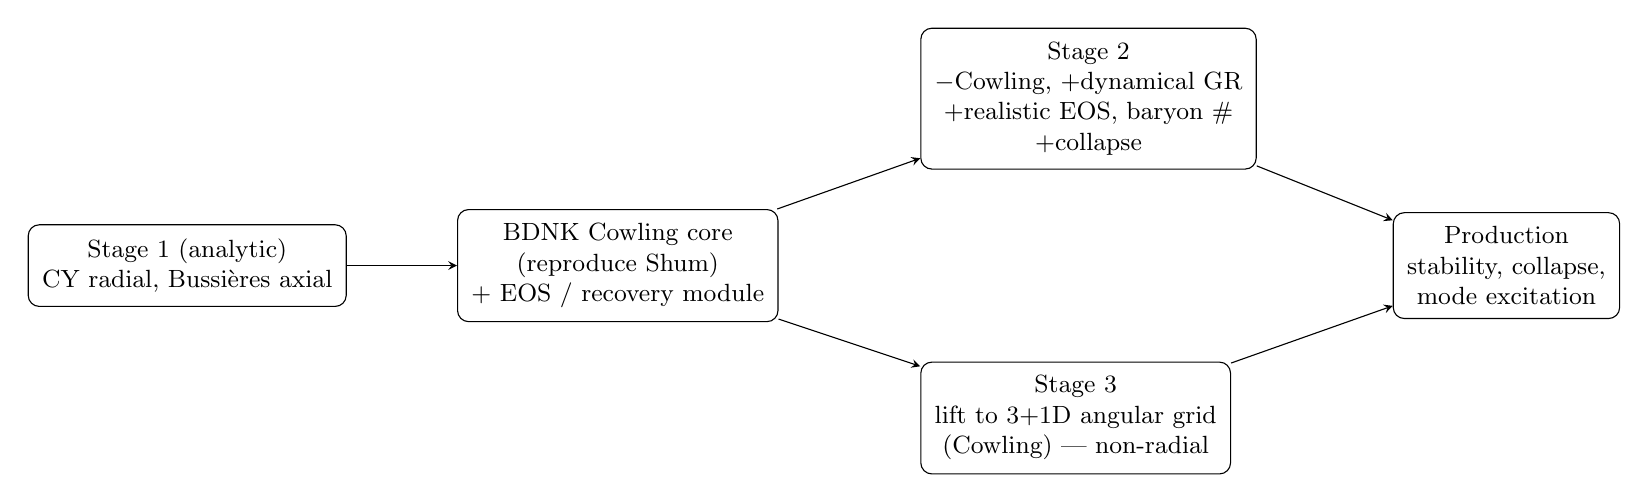
\begin{tikzpicture}[
  box/.style={draw, rounded corners, align=center, inner sep=5pt, font=\small},
  >=stealth
]
\node[box] (analytic) {Stage 1 (analytic)\\CY radial, Bussi\`eres axial};
\node[box, right=14mm of analytic] (core) {BDNK Cowling core\\(reproduce Shum)\\$+$ EOS / recovery module};
\node[box, above right=5mm and 18mm of core] (s2) {Stage 2\\$-$Cowling,\ $+$dynamical GR\\$+$realistic EOS, baryon \#\\$+$collapse};
\node[box, below right=5mm and 18mm of core] (s3) {Stage 3\\lift to $3{+}1$D angular grid\\(Cowling) --- non-radial};
\node[box, right=78mm of core] (prod) {Production\\stability, collapse,\\mode excitation};
\draw[->] (analytic) -- (core);
\draw[->] (core) -- (s2);
\draw[->] (core) -- (s3);
\draw[->] (s2) -- (prod);
\draw[->] (s3) -- (prod);
\end{tikzpicture}}
\caption{Dependency structure. The BDNK Cowling (the Shum et al.\
reproduction, with the shared equation-of-state and primitive-recovery module) is
the trunk; Stages~2 and~3 are independent forks that recombine at production.}
\label{fig:dep}
\end{figure}

\section{Stage 1 --- Reproduce known results}
Separate the analytic reproductions from the numerical one. The two analytic
targets are inexpensive frequency-domain (shooting / eigenvalue) calculations and
should come first, because they furnish validated linear benchmarks for every
later stage. Reproduce the Caballero--Yunes radial spectrum \emph{including} the
heat-conduction sector---not merely bulk and shear---because that is the sole
nontrivial instability channel and is where the Stage-2 stability question
resides. Reproduce the Bussi\`eres--Redondo-Yuste axial spectrum to fix the
viscous mode families to be sought later in the time domain.

The numerical reproduction of Shum et al.\ is the core engine. Treat reaching
their restricted stable-parameter window and recovering their quasinormal-mode
frequencies and fundamental-mode decay rate as the acceptance test for the trunk.

\section{Stage 2 --- $1{+}1$D dynamical GR, realistic EOS, collapse}

\paragraph{General-relativistic coupling.}
The dynamical-spacetime viscous (Israel--Stewart)
infrastructure already developed by the Palenzuela--Bezares group can be reused by
substituting the BDNK stress tensor for the Israel--Stewart one inside an existing
Valencia-conservative plus BSSN/CCZ4 (or Misner--Sharp, in radial gauge) setup;
this is far cheaper than new numerical relativity. Apparent-horizon finding in
spherical symmetry is a one-dimensional root find for the marginally trapped
surface. Carry constraint damping explicitly, given the known sensitivity of
constraint propagation in first-order viscous systems \cite{FantiniRubio2025}.

\paragraph{Shocks and collapse.}
Use high-resolution shock capturing (an HLL-type or central / Kurganov--Tadmor
scheme with high-order reconstruction) on the advective operator, with an IMEX
Runge--Kutta integrator for the relaxation-type $\tau$ terms when they become stiff
(small viscosity or large coefficients), positivity-preserving limiting, and a
hardened atmosphere---the stellar surface is the principal recovery-failure site.
Seed collapse explicitly through depleted pressure, an inward velocity, or a
configuration just beyond $M_{\max}$.

\paragraph{Heat conduction in scope.}
The first physics question---whether full GR coupling changes radial
stability---most plausibly has a nontrivial answer in the heat-conduction channel,
the only channel Caballero--Yunes find unstable. Baryon-number conservation and the
dissipative heat / number flux therefore belong in Stage~2 from the outset, with
the linear limit checked against the Caballero--Yunes criterion as a combined
physics-and-frame test.

\paragraph{Frames.}
Evolve in at least two distinct hydrodynamic-frame parametrizations. A genuine
instability persists across frames and converges under refinement at fixed, small
Knudsen-like parameter $\mathrm{Kn}\sim\tau\omega$; a frame artifact does not. Fix
the frame-invariant observables (mode frequencies, damping times, collapse time)
in advance so the cross-frame comparison is well posed.

\medskip
\noindent These choices map directly onto the two Stage-2 questions: heat
conduction and multi-frame evolution for the stability question, and the
shock-capturing collapse machinery for the effect of viscosity on collapse.

\section{Stage 3 --- $3{+}1$D Cowling, non-radial modes}
The same recovery module applies, augmented with the angular-derivative gradient
terms (this is the content of the ``$3{+}1$D polytropic recovery''); the two-sphere
formulation of first-order viscous hydrodynamics \cite{KeeblePretorius2025} is a
useful precursor for the angular sector. Validate the linear axial sector directly
against Bussi\`eres et al.: seed small $\ell\ge 2$ axial perturbations, extract the
quasinormal modes, and confirm recovery of the viscosity-driven families with no
perfect-fluid counterpart. Only then proceed to the polar sector and mode coupling,
to address whether new modes appear, whether stability is modified, and how the
non-radial modes are excited. This stage is the nonlinear, time-domain counterpart
of the Bussi\`eres frequency-domain analysis, which supplies its correctness check.

\section{Cross-cutting choices and additions}
\begin{itemize}
\item \textbf{Convergence and constraint monitors as first-class outputs.} The
BDNK--numerical-relativity literature is judged on self-convergence and constraint
preservation; build the monitors before the physics runs.

\item \textbf{An Israel--Stewart comparison run}  is the
cleanest way to argue that a given feature is physical rather than a BDNK frame
artifact, and it connects to existing merger results \cite{ChabanovRezzolla2023}.

\item \textbf{Transport-coefficient decision, made early.} Dimensionless /
parametrized $(\eta,\zeta,\kappa,\tau)$ for the methods papers versus physical
dense-matter coefficients for the astrophysics result are different deliverables;
decide which Stage~2 is.

\item \textbf{Initial data.} A static viscous star is simply a TOV solution
(dissipation vanishes in equilibrium), so the content lies entirely in how the
out-of-equilibrium perturbation or collapse is seeded.

\item \textbf{Gravitational-wave extraction} (Cowling $\to$ dynamical for non-radial
modes) is the natural fourth stage and is left out of the present scope.
\end{itemize}

\section{Phasing with validation gates}
\begin{enumerate}
\item Analytic benchmarks (Caballero--Yunes radial including heat conduction;
Bussi\`eres axial). \emph{Gate:} both spectra reproduced.
\item BDNK Cowling core plus shared equation-of-state / recovery module
(polytropic $\to$ ideal $\to$ tabulated). \emph{Gate:} Shum quasinormal-mode
frequencies, decay rate, and stable-parameter window reproduced.
\item Stage~2: dynamical GR, baryon number, shock capturing, multi-frame.
\emph{Gate:} linear radial spectrum matches the Caballero--Yunes criterion across
frames; convergent collapse with apparent-horizon formation.
\item Stage~3: lift to $3{+}1$D Cowling. \emph{Gate:} linear axial spectrum matches
the Bussi\`eres viscous mode families.
\item Production: heat-conduction stability under GR; viscous collapse dynamics;
non-radial mode content and excitation.
\end{enumerate}

\begin{thebibliography}{9}
\bibitem{CaballeroYunes2025} D.~A.~Caballero and N.~Yunes,
\emph{Neutron star radial perturbations for causal, viscous, relativistic fluids},
Phys. Rev. D \textbf{112}, 063050 (2025), arXiv:2506.09149.

\bibitem{Bussieres2026} S.~Bussi\`eres, J.~Redondo-Yuste, J.~J.~Ortega G\'omez, and
V.~Cardoso, \emph{Axial Oscillations of Viscous Neutron Stars}, arXiv:2604.13208
(2026).

\bibitem{Shum2026} H.~L.~H.~Shum, F.~Abalos, Y.~Bea, M.~Bezares, P.~Figueras, and
C.~Palenzuela, \emph{Neutron star evolution with the
Bemfica--Disconzi--Noronha--Kovtun viscous hydrodynamics framework}, Phys. Rev. D
\textbf{113}, 084029 (2026), arXiv:2509.15303.

\bibitem{RedondoYuste2025} J.~Redondo-Yuste, \emph{Perturbations of relativistic
dissipative stars}, Class. Quantum Grav. \textbf{42}, 075012 (2025),
arXiv:2411.16841.

\bibitem{FantiniRubio2025} D.~Fantini and M.~E.~Rubio, \emph{Constraint evolution in
first-order viscous relativistic fluids}, Phys. Rev. D \textbf{112}, 063038 (2025).

\bibitem{PandyaMostPretorius2022} A.~Pandya, E.~R.~Most, and F.~Pretorius,
\emph{Causal, stable first-order viscous relativistic hydrodynamics with ideal gas
microphysics}, Phys. Rev. D \textbf{106}, 123036 (2022).

\bibitem{KeeblePretorius2025} L.~S.~Keeble and F.~Pretorius, \emph{First-order
viscous relativistic hydrodynamics on the two-sphere}, Phys. Rev. D \textbf{112},
124034 (2025).

\bibitem{ChabanovRezzolla2023} M.~Chabanov and L.~Rezzolla, \emph{Numerical
modelling of bulk viscosity in neutron stars}, arXiv:2311.13027 (2023).
\end{thebibliography}

\end{document}
